% !TeX program = xelatex
% A题前三问论文初稿：基于仓库 results/problem1--3 与 code/problem1--3 整理。
\documentclass[UTF8,a4paper,12pt]{ctexart}

\usepackage[left=2.54cm,right=2.54cm,top=2.54cm,bottom=2.54cm]{geometry}
\usepackage{amsmath,amssymb,mathtools,bm}
\usepackage{booktabs,longtable,array,multirow,tabularx}
\usepackage{graphicx,float,subcaption}
\usepackage{caption}
\usepackage{algorithm2e}
\usepackage{xcolor}
\usepackage{enumitem}
\usepackage{listings}
\usepackage{hyperref}
\usepackage{titlesec}
\usepackage{fancyhdr}

\IfFontExistsTF{SimSun}{\setCJKmainfont{SimSun}}{}
\IfFontExistsTF{Times New Roman}{\setmainfont{Times New Roman}}{}
\linespread{1.0}\selectfont
\setlength{\parindent}{2em}
\setlength{\parskip}{0pt}
\setcounter{secnumdepth}{3}
\setcounter{tocdepth}{2}
\renewcommand{\theequation}{\arabic{equation}}
\numberwithin{equation}{section}

\captionsetup{font={small},labelfont=bf,labelsep=quad,skip=2pt,aboveskip=2pt,belowskip=0pt}
\setlength{\abovecaptionskip}{2pt}
\setlength{\belowcaptionskip}{0pt}
\setlength{\floatsep}{4pt plus 1pt minus 1pt}
\setlength{\textfloatsep}{4pt plus 1pt minus 1pt}
\setlength{\intextsep}{4pt plus 1pt minus 1pt}

\ctexset{
  section={format=\centering\bfseries\fontsize{14pt}{18pt}\selectfont, name={,、}, number=\chinese{section}, aftername=\quad, beforeskip=14pt, afterskip=8pt},
  subsection={format=\bfseries\fontsize{12pt}{16pt}\selectfont, beforeskip=10pt, afterskip=5pt},
  subsubsection={format=\bfseries\fontsize{12pt}{16pt}\selectfont, beforeskip=8pt, afterskip=4pt}
}
\pagestyle{fancy}
\fancyhf{}
\cfoot{\thepage}
\renewcommand{\headrulewidth}{0pt}

\lstset{basicstyle=\ttfamily\small,breaklines=true,frame=single,columns=fullflexible,numbers=left,numberstyle=\tiny,showstringspaces=false}
\hypersetup{colorlinks=true,linkcolor=black,citecolor=black,urlcolor=black,pdftitle={药材热风烘干过程的热质耦合建模与数值模拟}}

\begin{document}

\begin{center}
  {\fontsize{14pt}{18pt}\selectfont\bfseries 药材热风烘干过程的热质耦合建模与数值模拟}\par\vspace{10pt}
  {\fontsize{14pt}{18pt}\selectfont\bfseries 摘要}
\end{center}

本文围绕中药材热风烘干过程，建立一维径向热传导与水分扩散模型，用数值仿真刻画药材内部温度场和干基含水率场随时间与半径的变化规律，并进一步求解达到全截面含水率阈值所需的烘干时长。针对圆柱形药材长度明显大于半径的特点，本文忽略轴向和端面效应，将药材截面简化为轴对称径向传递问题；外部烘房温湿边界由附件数据插值得到，表面采用第三类换热、传质边界。

\noindent \textbf{针对问题一，}在预热平衡阶段，题设给出的密度、比热容和热导率均为常数，水分扩散系数只与含水率有关。因此温度场与水分场可在同一径向有限体积框架下分别求解。本文采用守恒型有限体积离散与 BDF 隐式积分，内部计算网格取 $0.0025\rm\,cm$，再按题目要求输出 $1\rm\,s$ 和 $0.1\rm\,cm$ 间隔结果。计算得到 $1800\rm\,s$ 时中心和表面温度分别为 $33.5753^\circ\mathrm C$、$36.7856^\circ\mathrm C$，中心和表面水分浓度分别为 $2.5500\rm\,kg/kg$、$1.5102\rm\,kg/kg$。结果表明，预热阶段热扰动已传入大部分半径，而显著脱水仍集中在表层。

\noindent \textbf{针对问题二，}在问题一模型的基础上，引入附录3中随水分浓度变化的密度、比热容、热导率以及随温度和水分共同变化的扩散系数，建立温度与水分双向耦合的非线性模型。每个时间步内采用 Picard 定点迭代更新物性并隐式求解两场。3 h 时，药材中心和表面温度分别为 $49.8531^\circ\mathrm C$、$49.9692^\circ\mathrm C$，中心和表面水分浓度分别为 $1.7625\rm\,kg/kg$、$0.9993\rm\,kg/kg$。与问题一相比，温度场逐渐接近烘房温度，水分场仍保持明显的内外梯度，说明干燥过程后续主要受内部水分扩散控制。

\noindent \textbf{针对问题三，}将问题二的耦合模型延拓到完整烘干过程，并以全截面水分浓度均低于 $0.15\rm\,kg/kg$ 作为停机判据。由于附件1仅给出前 4 h 的环境数据，本文在 4 h 后采用附件1末值恒定外推作为恒温干燥段边界条件。计算得到烘干终止时间为 $198210\rm\,s$，即 $55.0583\rm\,h$。终止时刻全精度中心含水率为 $0.149998\rm\,kg/kg$，满足阈值条件；论文表中显示为 $0.1500$ 是四舍五入结果。模型检验显示问题一加密网格结果对四位小数输出影响很小，问题二和问题三所有 Picard 时间步均收敛；但第三问结果对 4 h 后边界外推具有较强依赖，需在工艺解释中明确该边界假设。

\noindent \textbf{关键词：}热风烘干\quad 径向有限体积法\quad 热质耦合\quad Picard 迭代\quad 干基含水率

\section{问题重述}
\subsection{问题背景}
中药材烘干是影响药材品质、生产效率与能耗的重要工序。热风烘干通常包括预热平衡和恒温干燥两个阶段：前者以药材升温和表层水分响应为主，后者以持续脱水为主。传统试验优化需要较长周期和较高成本，因此有必要建立能够反映药材内部温度和水分迁移规律的数学模型，用仿真结果辅助烘干工艺参数分析。

题目将药材近似为长 $25\rm\,cm$、半径 $2\rm\,cm$ 的圆柱体，给出初始温度、初始干基含水率、烘房温湿边界和若干经验物性公式。本文仅讨论前三问，不考虑第四问中的半径收缩。

\subsection{已知数据、条件与约束}
药材初始温度为 $28^\circ\mathrm C$，初始水分浓度为 $2.55\rm\,kg/kg$，初始状态在空间上均匀分布。附件1给出了烘房环境温度 $T_\infty(t)$ 与环境水分浓度 $C_\infty(t)$ 的时间序列。问题一使用附录2参数，问题二和问题三使用附录3经验公式。题目要求结果按指定时刻和指定径向位置列入论文表格，并将完整时空网格写入对应 Excel 文件，数值保留四位小数。

\subsection{逐问任务}
问题一要求在 $0$ 到 $1800\rm\,s$ 的预热平衡阶段内，建立药材温度和水分浓度的时空变化模型，给出表1和表2，并输出 $1\rm\,s$ 与 $0.1\rm\,cm$ 分辨率的完整结果。

问题二要求建立预热平衡和恒温干燥全过程的温度、水分耦合模型，并给出前 $3\rm\,h$ 内每隔 $0.5\rm\,h$、半径方向 $0,0.5,1,1.5,2\rm\,cm$ 处的温度和水分浓度。

问题三要求在问题二模型基础上继续积分，求药材各处水分浓度均低于 $0.15\rm\,kg/kg$ 所需的烘干时间，并输出每隔 $6\rm\,h$ 及终止时刻的水分浓度分布。

\section{问题分析}
\subsection{问题一分析}
问题一处于预热平衡阶段，时间较短，外部边界由附件1在 $0$ 到 $1800\rm\,s$ 内直接插值得到。附录2中 $\rho,c_p,k$ 为常数，水分扩散系数 $D$ 只依赖 $C$，因此温度方程与水分方程在数学上解耦。该问的核心是用足够稳定的径向扩散模型解释表面先升温、先失水，中心响应滞后的现象，并给后续耦合模型提供统一的几何、边界和离散框架。

\subsection{问题二分析}
问题二在几何与边界形式上继承问题一，但物性公式发生变化：$\rho,c_p,k$ 随水分浓度改变，$D$ 同时依赖水分浓度与绝对温度。于是水分场影响温度方程中的物性参数，温度场又影响水分扩散系数，二者形成非线性双向耦合。该问的建模重点是每个时间步内同步更新物性并保证耦合迭代收敛。

\subsection{问题三分析}
问题三不再只报告固定时间窗口，而是把问题二的耦合模型延拓到烘干结束。终止条件为药材所有径向位置的水分浓度均低于 $0.15\rm\,kg/kg$，因此应监测全截面水分最大值。由于中心点失水最慢，终止时间通常由中心含水率决定。该问的主要不确定性来自附件1只给出前 $4\rm\,h$ 环境数据，本文采用末值恒定外推作为恒温干燥段边界，并在模型评价中说明该假设的影响。

\section{模型假设}
\begin{enumerate}[label=\arabic*.,leftmargin=2.5em]
  \item 药材可视为长圆柱体，长度远大于半径，忽略轴向传递和端面效应，只考虑一维径向传热、传质。
  \item 初始时刻药材内部温度和干基含水率均匀分布，分别为 $28^\circ\mathrm C$ 和 $2.55\rm\,kg/kg$。
  \item 药材表面与烘房热风之间采用第三类换热和第三类传质边界；烘房内温度与水分浓度空间均匀。
  \item 问题一至问题三均不考虑半径收缩，半径固定为 $R=0.02\rm\,m$。
  \item 附录3未另给对流换热系数和对流传质系数，问题二和问题三沿用附录2参数 $h=25\rm\,W/(m^2\cdot K)$、$h_m=8\times10^{-7}\rm\,m/s$。
  \item 题目未提供显式蒸发潜热源项所需参数，本文在题设经验物性体系下不额外加入相变源项。
  \item 问题三中 $4\rm\,h$ 后的恒温干燥边界取附件1末时刻环境温度和环境水分浓度并保持不变。
\end{enumerate}

\section{符号说明}
\begin{table}[H]
  \centering
  \caption{主要符号说明}
  \begin{tabular}{>{\centering\arraybackslash}p{0.18\textwidth}p{0.55\textwidth}>{\centering\arraybackslash}p{0.17\textwidth}}
    \toprule
    符号 & 含义 & 单位\\ \midrule
    $r$ & 到药材中心轴的径向距离 & m\\
    $R$ & 药材半径，前三问取 $0.02$ & m\\
    $t$ & 烘干时间 & s\\
    $T(r,t)$ & 药材内部温度 & $^\circ\mathrm C$\\
    $T_K$ & 绝对温度，$T_K=T+273.15$ & K\\
    $C(r,t)$ & 干基水分浓度 & kg/kg\\
    $T_\infty(t)$ & 烘房环境温度 & $^\circ\mathrm C$\\
    $C_\infty(t)$ & 烘房环境水分浓度 & kg/kg\\
    $\rho(C)$ & 密度 & kg/m$^3$\\
    $c_p(C)$ & 比热容 & J/(kg$\cdot$K)\\
    $k(C)$ & 热导率 & W/(m$\cdot$K)\\
    $D(C,T)$ & 有效水分扩散系数 & m$^2$/s\\
    $h$ & 对流换热系数 & W/(m$^2\cdot$K)\\
    $h_m$ & 对流传质系数 & m/s\\
    $t_{\rm end}$ & 达到水分阈值所需烘干时间 & h\\
    \bottomrule
  \end{tabular}
\end{table}

\section{数据预处理与数值离散基础}
\subsection{边界数据插值}
附件1给出离散时刻的烘房温度和环境水分浓度。为在任意时间步调用边界条件，本文采用分段线性插值：
\begin{equation}
  y_\infty(t)=y_j+\frac{y_{j+1}-y_j}{t_{j+1}-t_j}(t-t_j),
  \qquad t_j\le t\le t_{j+1},
\end{equation}
其中 $y$ 可表示 $T$ 或 $C$。问题一和问题二报告窗口均位于附件1覆盖范围内，因此直接由式(5.1)确定边界值。问题三在 $t>4\rm\,h$ 时采用末值保持：
\begin{equation}
  T_\infty(t)=T_\infty(4{\rm h}),\qquad C_\infty(t)=C_\infty(4{\rm h}),\qquad t>4{\rm h}.
\end{equation}

\subsection{几何简化依据}
径向模型是否合理可由 Biot 数和扩散尺度共同判断。热 Biot 数和质 Biot 数定义为
\begin{equation}
  Bi_T=\frac{hR}{k},\qquad Bi_C=\frac{h_mR}{D(C_0)}.
\end{equation}
问题一参数下有 $Bi_T\approx1.389$、$Bi_C\approx3.24$，二者均大于 $0.1$，说明内部梯度不可忽略。另一方面，$1800\rm\,s$ 内热扩散尺度和水分扩散尺度为
\begin{equation}
  l_T=\sqrt{\alpha t},\qquad l_C=\sqrt{D(C_0)t},\qquad \alpha=\frac{k}{\rho c_p}.
\end{equation}
代入参数得 $l_T\approx1.74\rm\,cm$、$l_C\approx0.30\rm\,cm$，均小于圆柱半长 $12.5\rm\,cm$，故忽略端面效应具有合理性。

\subsection{径向有限体积离散}
取单位长度圆柱截面，节点 $r_i=i\Delta r$，控制体体积和界面面积为
\begin{equation}
  V_i=\pi\left(r_{i+1/2}^2-r_{i-1/2}^2\right),\qquad
  A_{i+1/2}=2\pi r_{i+1/2}.
\end{equation}
对一般扩散方程
\begin{equation}
  a(u)\frac{\partial u}{\partial t}
  =\frac1r\frac{\partial}{\partial r}\left(r\,b(u)\frac{\partial u}{\partial r}\right),
\end{equation}
内部节点的半离散形式写为
\begin{equation}
  a_iV_i\frac{du_i}{dt}
  =b_{i-1/2}A_{i-1/2}\frac{u_{i-1}-u_i}{\Delta r}
  +b_{i+1/2}A_{i+1/2}\frac{u_{i+1}-u_i}{\Delta r}.
\end{equation}
中心控制体因 $A_{-1/2}=0$ 自然满足对称零通量条件。表面控制体额外加入对流通量，从而实现第三类边界。

\section{问题一模型的建立与求解}
\subsection{本问任务与前文承接}
问题一要求在固定半径圆柱内计算 $0$ 到 $1800\rm\,s$ 预热平衡阶段的温度场和水分场。本问采用附录2常物性参数和 $D(C)$ 经验公式，是后续问题二、问题三热质耦合模型的基础版本。

\subsection{模型建立}
温度场满足径向 Fourier 热传导方程：
\begin{equation}
  \rho c_p\frac{\partial T}{\partial t}
  =\frac1r\frac{\partial}{\partial r}
  \left(kr\frac{\partial T}{\partial r}\right),
  \qquad 0<r<R.
\end{equation}
水分场满足守恒型 Fick 扩散方程：
\begin{equation}
  \frac{\partial C}{\partial t}
  =\frac1r\frac{\partial}{\partial r}
  \left[rD(C)\frac{\partial C}{\partial r}\right],
  \qquad
  D(C)=7\times10^{-9}\exp\left(-\frac{0.89}{C}\right).
\end{equation}
初始条件为
\begin{equation}
  T(r,0)=28,\qquad C(r,0)=2.55.
\end{equation}
中心对称边界为
\begin{equation}
  \left.\frac{\partial T}{\partial r}\right|_{r=0}=0,\qquad
  \left.\frac{\partial C}{\partial r}\right|_{r=0}=0.
\end{equation}
表面 Robin 边界为
\begin{equation}
  -k\left.\frac{\partial T}{\partial r}\right|_{r=R}
  =h\left[T(R,t)-T_\infty(t)\right],
\end{equation}
\begin{equation}
  -D(C_s)\left.\frac{\partial C}{\partial r}\right|_{r=R}
  =h_m\left[C(R,t)-C_\infty(t)\right].
\end{equation}
由于本问 $D$ 不依赖温度，$\rho,c_p,k$ 均为常数，因此式(6.1)和式(6.2)可以分别求解。

\subsection{模型求解}
本问采用一维径向有限体积法进行空间离散，并用 BDF 隐式方法推进时间。内部计算网格取 $\Delta r=0.0025\rm\,cm$，最后插值或抽取至题目要求的 $0.1\rm\,cm$ 输出网格。

\begin{algorithm}[H]
  \SetAlgoLined
  \KwIn{几何参数 $R$，初值 $T_0,C_0$，附件1边界序列，附录2物性参数}
  \KwOut{$0$ 到 $1800\rm\,s$ 内各输出点的 $T(r,t)$ 与 $C(r,t)$}
  构造径向有限体积网格和控制体几何量\;
  对附件1环境温度和环境水分浓度建立线性插值函数\;
  分别组装温度方程和水分方程的隐式时间积分右端\;
  用 BDF 积分至 $1800\rm\,s$\;
  抽取题目指定时间和半径位置的结果，保留四位小数\;
  \caption{问题一求解流程}
\end{algorithm}

\subsection{结果分析}
表\ref{tab:q1-temp} 和表\ref{tab:q1-moist} 给出了问题一论文抽样结果。温度表明，$1800\rm\,s$ 时药材表面已升至 $36.7856^\circ\mathrm C$，中心为 $33.5753^\circ\mathrm C$，说明热量已经传入内部但仍存在径向温差。水分表明，同一时刻表面水分浓度降至 $1.5102\rm\,kg/kg$，中心仍为 $2.5500\rm\,kg/kg$，脱水主要集中于表层。

\begin{table}[H]
  \centering
  \caption{30分钟内药材的温度 $/^\circ\mathrm C$}
  \label{tab:q1-temp}
  \begin{tabular}{rrrrrr}
    \toprule
    时间/s & 0 cm & 0.5 cm & 1 cm & 1.5 cm & 2 cm\\ \midrule
    100 & 28.0001 & 28.0003 & 28.0040 & 28.0327 & 28.1801\\
    300 & 28.0408 & 28.0635 & 28.1514 & 28.3681 & 28.8489\\
    600 & 28.4533 & 28.5360 & 28.8039 & 29.3159 & 30.1652\\
    900 & 29.3243 & 29.4583 & 29.8755 & 30.6161 & 31.7304\\
    1200 & 30.5427 & 30.7098 & 31.2223 & 32.1126 & 33.4276\\
    1500 & 31.9957 & 32.1867 & 32.7660 & 33.7463 & 35.1203\\
    1800 & 33.5753 & 33.7720 & 34.3642 & 35.3621 & 36.7856\\
    \bottomrule
  \end{tabular}
\end{table}

\begin{table}[H]
  \centering
  \caption{30分钟内药材的水分浓度 $/\rm kg\cdot kg^{-1}$}
  \label{tab:q1-moist}
  \begin{tabular}{rrrrrr}
    \toprule
    时间/s & 0 cm & 0.5 cm & 1 cm & 1.5 cm & 2 cm\\ \midrule
    100 & 2.5500 & 2.5500 & 2.5500 & 2.5500 & 2.2471\\
    300 & 2.5500 & 2.5500 & 2.5500 & 2.5492 & 2.0508\\
    600 & 2.5500 & 2.5500 & 2.5500 & 2.5353 & 1.8770\\
    900 & 2.5500 & 2.5500 & 2.5497 & 2.5045 & 1.7547\\
    1200 & 2.5500 & 2.5500 & 2.5482 & 2.4646 & 1.6586\\
    1500 & 2.5500 & 2.5499 & 2.5445 & 2.4206 & 1.5787\\
    1800 & 2.5500 & 2.5497 & 2.5383 & 2.3755 & 1.5102\\
    \bottomrule
  \end{tabular}
\end{table}

\begin{figure}[H]
  \centering
  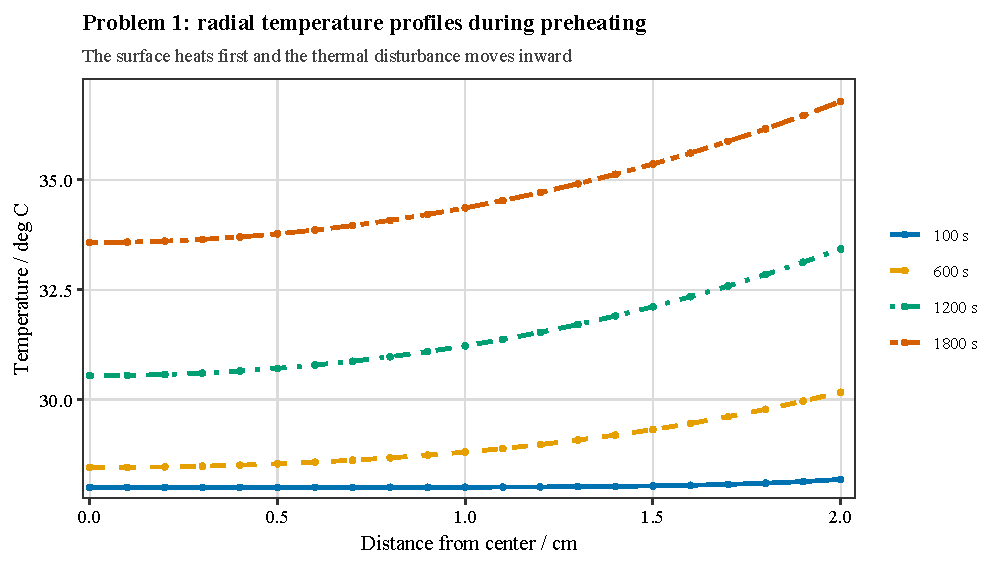
\includegraphics[width=0.92\textwidth]{../../results/problem1/figures/problem1_temperature_radial_profiles.pdf}
  \caption{问题一预热阶段不同时间的温度径向分布。曲线从中心到表面逐渐升高，且随时间整体上移，说明热量首先经表面对流进入药材并向中心传递。}
  \label{fig:q1-temperature-profiles}
\end{figure}

\begin{figure}[H]
  \centering
  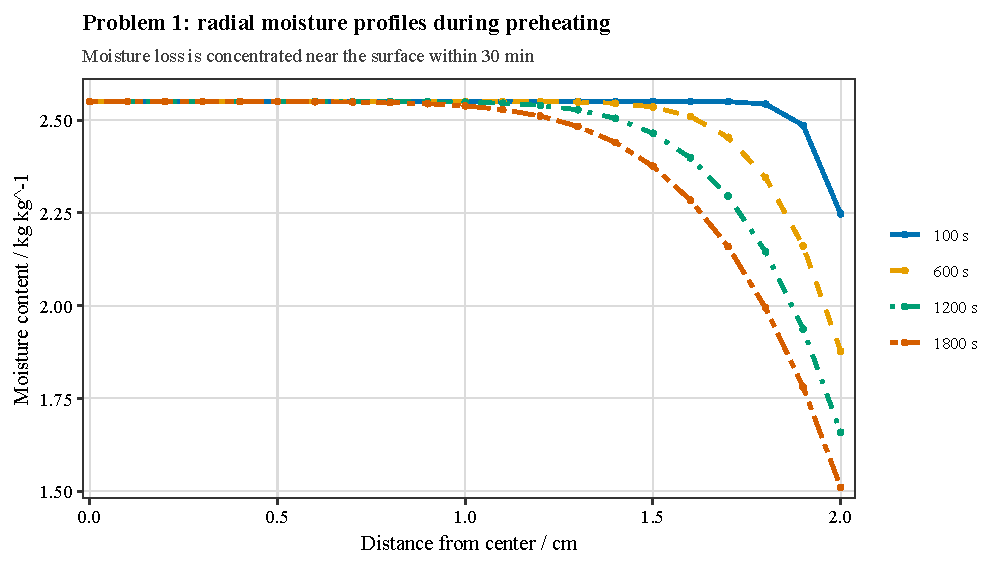
\includegraphics[width=0.92\textwidth]{../../results/problem1/figures/problem1_moisture_radial_profiles.pdf}
  \caption{问题一预热阶段不同时间的水分浓度径向分布。30 min 内中心附近水分浓度基本保持初值，主要降幅集中在近表面区域，体现水分扩散相对热扩散更慢。}
  \label{fig:q1-moisture-profiles}
\end{figure}

\subsection{本问小结与后续衔接}
问题一建立了固定半径下的径向有限体积模型，并验证了药材内部温度和含水率不能视为空间均匀。该问确定的几何简化、Robin 边界和径向离散方式被问题二继承；问题二在此基础上把常物性模型升级为随状态变化的耦合模型。

\section{问题二模型的建立与求解}
\subsection{本问任务与前文承接}
问题二继承问题一的圆柱径向模型和表面对流边界，但物性改用附录3公式，并要求输出 $0.5$ 到 $3.0\rm\,h$ 的温度和水分浓度分布。该问的新增难点是温度场和水分场相互耦合。

\subsection{模型建立}
附录3给出的状态相关物性为
\begin{equation}
  \rho(C)=650+128C,
\end{equation}
\begin{equation}
  c_p(C)=1450+\frac{2736C}{C+1},
\end{equation}
\begin{equation}
  k(C)=0.21+\frac{0.38C}{C+1},
\end{equation}
\begin{equation}
  D(C,T)=2.4\times10^{-3}\exp\left(-\frac{0.45}{C}\right)
  \exp\left(-\frac{3850}{T_K}\right),\qquad T_K=T+273.15.
\end{equation}
温度方程变为
\begin{equation}
  \rho(C)c_p(C)\frac{\partial T}{\partial t}
  =\frac1r\frac{\partial}{\partial r}
  \left[rk(C)\frac{\partial T}{\partial r}\right].
\end{equation}
水分方程为
\begin{equation}
  \frac{\partial C}{\partial t}
  =\frac1r\frac{\partial}{\partial r}
  \left[rD(C,T)\frac{\partial C}{\partial r}\right].
\end{equation}
初始条件与中心边界沿用问题一。表面边界为
\begin{equation}
  -k(C_s)\left.\frac{\partial T}{\partial r}\right|_{r=R}
  =h\left[T(R,t)-T_\infty(t)\right],
\end{equation}
\begin{equation}
  -D(C_s,T_s)\left.\frac{\partial C}{\partial r}\right|_{r=R}
  =h_m\left[C(R,t)-C_\infty(t)\right].
\end{equation}

\subsection{模型求解}
问题二采用 $\Delta r=0.1\rm\,cm$、$\Delta t=1\rm\,s$，空间算子按径向有限体积形式离散，时间推进采用 backward-Euler 隐式格式。为处理 $T$ 与 $C$ 的双向耦合，每个时间步内执行 Picard 迭代。迭代容差取 $10^{-8}$，最大迭代次数取 8。

\begin{algorithm}[H]
  \SetAlgoLined
  \KwIn{上一时刻 $T^n,C^n$，附件1边界，附录3物性公式}
  \KwOut{下一时刻 $T^{n+1},C^{n+1}$}
  令 $T^{(0)}=T^n,\ C^{(0)}=C^n$\;
  \For{$m=0,1,\ldots$}{
    由 $C^{(m)}$ 计算 $\rho,c_p,k$，隐式求解温度方程得 $T^{(m+1)}$\;
    由 $T^{(m+1)},C^{(m)}$ 计算 $D$，隐式求解水分方程得 $C^{(m+1)}$\;
    若 $\max|T^{(m+1)}-T^{(m)}|$ 和 $\max|C^{(m+1)}-C^{(m)}|$ 均小于容差，则停止迭代\;
  }
  \Return $T^{n+1},C^{n+1}$\;
  \caption{问题二单时间步 Picard 耦合迭代}
\end{algorithm}

完整计算中 $10800$ 个时间步全部收敛，单步最大 Picard 迭代次数为 3，说明当前时间步和耦合容差能够稳定求解前 $3\rm\,h$ 过程。

\subsection{结果分析}
表\ref{tab:q2-temp} 和表\ref{tab:q2-moist} 给出了问题二结果。药材温度在前 $2\rm\,h$ 快速升高，随后逐渐接近烘房温度，$3\rm\,h$ 时中心与表面温差仅约 $0.1161^\circ\mathrm C$。水分浓度下降明显慢于温度均衡，$3\rm\,h$ 时中心仍为 $1.7625\rm\,kg/kg$，表面为 $0.9993\rm\,kg/kg$，说明全程烘干时长主要由内部水分扩散控制。

\begin{table}[H]
  \centering
  \caption{3小时内药材的温度 $/^\circ\mathrm C$}
  \label{tab:q2-temp}
  \begin{tabular}{rrrrrr}
    \toprule
    时间/h & 0 cm & 0.5 cm & 1 cm & 1.5 cm & 2 cm\\ \midrule
    0.5 & 32.2156 & 32.4093 & 32.9956 & 33.9944 & 35.4528\\
    1.0 & 40.4246 & 40.5965 & 41.1034 & 41.9211 & 43.0399\\
    1.5 & 45.8786 & 45.9664 & 46.2235 & 46.6340 & 47.1669\\
    2.0 & 48.4679 & 48.5054 & 48.6151 & 48.7890 & 49.0171\\
    2.5 & 49.4751 & 49.4872 & 49.5212 & 49.5723 & 49.6666\\
    3.0 & 49.8531 & 49.8588 & 49.8779 & 49.9132 & 49.9692\\
    \bottomrule
  \end{tabular}
\end{table}

\begin{table}[H]
  \centering
  \caption{3小时内药材的水分浓度 $/\rm kg\cdot kg^{-1}$}
  \label{tab:q2-moist}
  \begin{tabular}{rrrrrr}
    \toprule
    时间/h & 0 cm & 0.5 cm & 1 cm & 1.5 cm & 2 cm\\ \midrule
    0.5 & 2.5499 & 2.5486 & 2.5246 & 2.3251 & 1.6440\\
    1.0 & 2.5246 & 2.4935 & 2.3564 & 2.0207 & 1.4661\\
    1.5 & 2.3841 & 2.3236 & 2.1321 & 1.7986 & 1.3418\\
    2.0 & 2.1684 & 2.1058 & 1.9205 & 1.6215 & 1.2243\\
    2.5 & 1.9536 & 1.8974 & 1.7320 & 1.4667 & 1.1088\\
    3.0 & 1.7625 & 1.7126 & 1.5655 & 1.3271 & 0.9993\\
    \bottomrule
  \end{tabular}
\end{table}

\subsection{本问小结与后续衔接}
问题二在问题一径向扩散框架上引入状态相关物性和 Picard 耦合迭代，得到前 $3\rm\,h$ 的温度、水分分布。结果显示温度场趋稳快于水分场，后续问题三可沿用同一耦合模型，把目标从固定时间输出改为达标停机时间求解。

\section{问题三模型的建立与求解}
\subsection{本问任务与前文承接}
问题三在问题二模型基础上求烘干结束时间。本文保持半径固定和附录3物性公式不变，仅将时间积分延长到全截面含水率达标，并输出水分浓度表。

\subsection{模型建立}
定义全截面最大水分浓度为
\begin{equation}
  C_{\max}(t)=\max_{0\le r\le R} C(r,t).
\end{equation}
烘干结束时间定义为
\begin{equation}
  t_{\rm end}=\inf\{t:C_{\max}(t)<0.15\}.
\end{equation}
由于表面直接与低湿热风接触，表面含水率最先降低；中心位置传质路径最长，通常决定 $C_{\max}(t)$。因此计算中仍检查所有离散径向节点，而不是只检查平均含水率。

问题三的控制方程、初始条件和边界形式均与问题二相同。唯一新增处理是 $4\rm\,h$ 后边界按式(5.2)保持恒定。该外推假设是第三问终止时间的主要边界条件。

\subsection{模型求解}
问题三采用与问题二相同的隐式径向离散和 Picard 耦合迭代，时间步取 $10\rm\,s$，每 $60\rm\,s$ 保存一次水分浓度输出。每一步完成耦合迭代后计算 $C_{\max}(t)$，一旦满足式(8.2)即停止。完整求解中 $19821$ 个时间步全部收敛，单步最大 Picard 迭代次数为 4。

\begin{algorithm}[H]
  \SetAlgoLined
  \KwIn{初值 $T_0,C_0$，附录3物性，附件1环境边界及末值外推规则}
  \KwOut{烘干结束时间 $t_{\rm end}$ 与水分浓度过程表}
  初始化 $t=0$，设置全截面水分浓度 $C(r,0)=2.55$\;
  \While{$\max_i C_i(t)\ge0.15$}{
    按问题二 Picard 迭代求解下一时间步 $T,C$\;
    若到达 $60\rm\,s$ 输出间隔，则记录水分浓度分布\;
    更新 $t$\;
  }
  输出 $t_{\rm end}$ 及终止时刻水分浓度\;
  \caption{问题三达标停机求解流程}
\end{algorithm}

\subsection{结果分析}
计算得到
\begin{equation}
  t_{\rm end}=198210\rm\,s=55.0583\rm\,h.
\end{equation}
终止时刻全精度最大水分浓度出现在中心点，数值为
\begin{equation}
  C_{\max}(t_{\rm end})=0.149998\rm\,kg/kg<0.15\rm\,kg/kg.
\end{equation}
因此表\ref{tab:q3-moist} 末行中心值显示为 $0.1500$ 是四舍五入结果，并不违反停机判据。

\begin{table}[H]
  \centering
  \caption{药材烘干过程的水分浓度 $/\rm kg\cdot kg^{-1}$}
  \label{tab:q3-moist}
  \begin{tabular}{rrrrrr}
    \toprule
    时间/h & 0 cm & 0.5 cm & 1 cm & 1.5 cm & 2 cm\\ \midrule
    6 & 1.0087 & 0.9797 & 0.8926 & 0.7449 & 0.5187\\
    12 & 0.4448 & 0.4314 & 0.3898 & 0.3115 & 0.0504\\
    18 & 0.2895 & 0.2822 & 0.2594 & 0.2155 & 0.0501\\
    24 & 0.2314 & 0.2264 & 0.2104 & 0.1787 & 0.0500\\
    30 & 0.2010 & 0.1970 & 0.1843 & 0.1587 & 0.0500\\
    36 & 0.1819 & 0.1786 & 0.1677 & 0.1458 & 0.0500\\
    42 & 0.1687 & 0.1657 & 0.1562 & 0.1367 & 0.0500\\
    48 & 0.1588 & 0.1562 & 0.1476 & 0.1298 & 0.0500\\
    54 & 0.1512 & 0.1487 & 0.1408 & 0.1244 & 0.0500\\
    55.0583 & 0.1500 & 0.1476 & 0.1398 & 0.1236 & 0.0500\\
    \bottomrule
  \end{tabular}
\end{table}

从表\ref{tab:q3-moist} 可见，表面含水率在 $12\rm\,h$ 左右已接近环境水分水平，而中心水分下降显著滞后。$48\rm\,h$ 时中心含水率仍高于阈值，直到 $55.0583\rm\,h$ 才首次低于 $0.15\rm\,kg/kg$。这说明以平均含水率或表面含水率作为停机依据会过早终止烘干，必须采用全截面判据。

\subsection{本问小结与后续衔接}
问题三将问题二模型延拓到完整烘干过程，得到在附件1末值恒定外推假设下的终止时间 $55.0583\rm\,h$。该结果可作为不考虑收缩时的基准烘干时长，并为第四问引入移动边界后的比较提供参照。

\section{模型检验与稳定性分析}
\subsection{数值收敛检验}
问题一采用细于输出网格的内部计算网格。将内部网格由 $0.005\rm\,cm$ 加密至 $0.0025\rm\,cm$ 后，论文抽样单元中温度最大变化约为 $1.1\times10^{-4}{}^\circ\mathrm C$，水分浓度最大变化约为 $5.6\times10^{-5}\rm\,kg/kg$，均小于四位小数输出的主要分辨尺度。

问题二和问题三采用隐式时间推进与 Picard 耦合迭代。问题二 $10800$ 个时间步全部收敛，最大迭代次数为 3；问题三 $19821$ 个时间步全部收敛，最大迭代次数为 4。该结果说明耦合迭代在当前参数下稳定。

\subsection{边界敏感性讨论}
问题三中 $4\rm\,h$ 后的烘房温湿边界并非由附件直接给出，而是按附件1末值恒定外推。由于 $t_{\rm end}=55.0583\rm\,h$，大部分积分时间都处于外推边界下，因此该终止时间应表述为“在附件1末值恒定外推假设下”的结果。

若用于最终竞赛论文，建议补做如下灵敏度表：将 $T_\infty(>4\rm\,h)$ 分别扰动 $\pm2^\circ\mathrm C$，将 $C_\infty(>4\rm\,h)$ 分别扰动 $\pm10\%$，比较 $t_{\rm end}$ 的变化量和相对变化率。由于当前仓库未包含原始附件文件，本文初稿不伪造敏感性数值，只在模型评价中明确该边界假设。

\subsection{物理合理性检验}
三个问题均呈现表面先响应、中心滞后的规律。问题一中表面升温和脱水均快于中心；问题二中温度场接近均匀后水分场仍保持梯度；问题三中表面含水率较早接近下界，而中心点控制最终停机时间。该趋势与圆柱径向扩散过程的物理直觉一致。

\section{模型评价}
\subsection{模型优点}
\begin{itemize}[leftmargin=2em]
  \item 模型从问题一到问题三保持同一径向守恒框架，能够自然衔接预热阶段、三小时窗口和达标停机问题。
  \item 问题二和问题三显式考虑了附录3中物性随水分和温度变化的非线性特征，并通过 Picard 迭代处理双向耦合。
  \item 采用全截面最大水分浓度作为问题三停机判据，避免用平均含水率或表面含水率低估烘干时间。
  \item 输出表格与 Excel 文件均按题目指定时间、空间分辨率和四位小数要求生成，便于复核。
\end{itemize}

\subsection{模型不足}
\begin{itemize}[leftmargin=2em]
  \item 模型未显式加入蒸发潜热源项，原因是题目未提供相变潜热及其耦合参数；该简化可能影响温度与水分迁移之间的真实耦合强度。
  \item 问题三 $4\rm\,h$ 后边界采用附件1末值恒定外推，终止时间对该外推假设可能敏感。
  \item 问题二主结果网格与题目输出网格一致，尚缺更细空间网格和相邻时间步的正式对照表。
\end{itemize}

\subsection{模型改进方向}
后续可从三方面改进：第一，若题目补充恒温干燥段设定值，应替换末值外推边界并重算问题三；第二，补充 $T_\infty$、$C_\infty$、$\Delta r$、$\Delta t$ 的灵敏度分析表，提高结论可信度；第三，在获得潜热或经验耦合参数后，可把蒸发潜热作为源项加入温度方程，进一步刻画烘干后期的热湿耦合。

\clearpage
\section*{AI 工具使用声明}
\addcontentsline{toc}{section}{AI 工具使用声明}
本参赛队在竞赛过程中使用了 AI 工具辅助代码调试、文字组织和格式检查；所有模型公式、参数取值、数值结果和结论均需由参赛队依据题目附件、程序输出和人工复核确认。

\clearpage
\begin{thebibliography}{99}
\addcontentsline{toc}{section}{参考文献}
\bibitem{cumcm2026a} 2026年全国大学生数学建模竞赛A题题目、附件及附录材料.
\end{thebibliography}

\clearpage
\appendix
\section{附录核心代码说明}
\subsection{Q1 核心代码接口}
\begin{lstlisting}[language=Python,caption={问题一求解主流程接口}]
# code/problem1/run_problem1.py
# 读取附件1边界数据，调用径向有限体积与 BDF 求解器，
# 输出 result1.xlsx 和论文表1、表2。
\end{lstlisting}

\subsection{Q2 核心代码接口}
\begin{lstlisting}[language=Python,caption={问题二 Picard 耦合求解接口}]
# code/problem2/solver.py
# solve_problem2(environment, config)
# 每个时间步内迭代更新 rho(C), cp(C), k(C), D(C,T)，
# 隐式求解温度场和水分场，记录耦合迭代收敛信息。
\end{lstlisting}

\subsection{Q3 核心代码接口}
\begin{lstlisting}[language=Python,caption={问题三达标停机接口}]
# code/problem3/solver.py
# solve_problem3(environment, config)
# 延拓问题二模型，直到 max(C(r,t)) < 0.15，
# 输出 t_end、result3.xlsx 和表5。
\end{lstlisting}

\end{document}
